% 给高中生的量子力学简介
% 双缝干涉|德布罗意波|量子力学|科普|平面波|球面波|玻尔原子

\subsection{简介}
对象: 对量子物理比较感兴趣的高中生. 数学要求不高, 物理图像为主.

\subsubsection{背景知识}
\begin{itemize}
\item 双缝干涉
\item 德布罗意物质波
\item 玻尔原子模型
\item 电子的双缝干涉
\end{itemize}

\subsubsection{一维波动力学(量子)}
\begin{itemize}
\item 概率波和波包
\item 自由高斯波包
\item 势垒散射\ 隧道效应
\item 无限深势阱
\end{itemize}

说明:
\begin{itemize}
\item 量子力学和波有什么关系?
\item 一维是什么?
\end{itemize}

\subsection{双缝干涉}

\subsubsection{平面波}

参考\upref{PWave}

一维平面波: 振幅, 波长 $\lambda$, 波速 $v$, 相位, 初相位 $\phi$
\begin{figure}[ht]
\centering
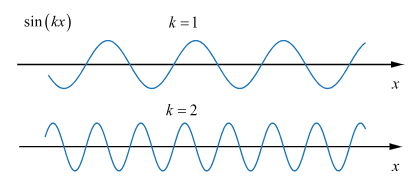
\includegraphics[width=9cm]{./figures/QMIntr2.png}
\caption{一维平面波 $\sin[k(x-vt) + \phi]$, 由负无穷延伸至正无穷.} \label{QMIntr_fig2}
\end{figure}

\begin{equation}
y = A \sin[k(x-vt) + \phi] = A \sin(kx - \omega t + \phi)
\end{equation}

\begin{equation}
\omega = kv
\end{equation}

\begin{equation}
\lambda = \frac{2\pi}{k}
\qquad
T = \frac{2\pi}{\omega}
\end{equation}

二维和三维平面波

\begin{figure}[ht]
\centering
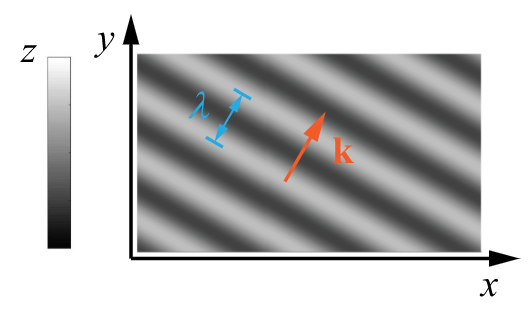
\includegraphics[width=7cm]{./figures/QMIntr6.png}
\caption{二维平面波} \label{QMIntr_fig6}
\end{figure}

\begin{equation}
s = A \cos(\bvec k \vdot \bvec r - \omega t + \varphi_0)
\end{equation}


\subsubsection{波的叠加与干涉}

波的叠加就是做加法, 相位差决定干涉结果

一维的波的叠加

什么是相干性?

二维:

\begin{figure}[ht]
\centering
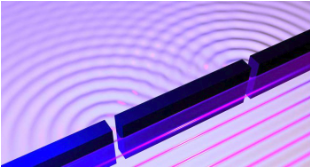
\includegraphics[width=7cm]{./figures/QMIntr4.png}
\caption{水波的干涉} \label{QMIntr_fig4}
\end{figure}

\begin{figure}[ht]
\centering
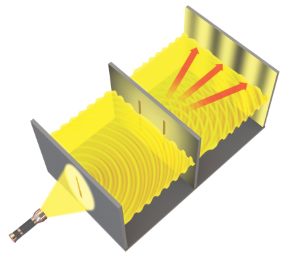
\includegraphics[width=6cm]{./figures/QMIntr5.png}
\caption{光的双缝干涉} \label{QMIntr_fig5}
\end{figure}

双缝干涉 \href{https://phet.colorado.edu/sims/html/wave-interference/latest/wave-interference_en.html}{PhET 演示}.

为什么用手电筒做不出? 不相干

\subsection{德布罗意物质波}

对于光子
\begin{equation}
\begin{aligned}
p &= mc
\\
E &= mc^2 = pc = h\nu = \frac{hc}{\lambda}
\end{aligned}
\end{equation}

德布罗意假设(两条不含 $c$ 的)
\begin{equation}
\lambda = \frac{h}{p}
\end{equation}

\begin{equation}
E = h\nu
\end{equation}

左边描述粒子性, 右边描述波动性

\subsection{概率波和波包}
参考\upref{QM0}

高斯波包\upref{QM0}, \href{http://wuli.wiki/apps/gausWP.html}{互动演示}

\subsection{电子的双缝干涉}

\begin{figure}[ht]
\centering
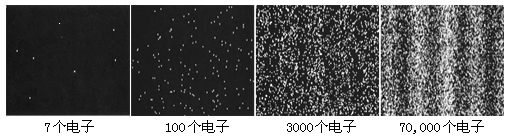
\includegraphics[width=12cm]{./figures/QMIntr3.png}
\caption{即使每次放出一个电子, 仍然会有干涉条纹} \label{QMIntr_fig3}
\end{figure}

\subsection{玻尔原子模型}
\pentry{圆周运动\upref{CMAD}, 牛顿第二定律\upref{New3}, 库仑力\upref{ClbFrc}}

参考\upref{BohrMd}

\begin{figure}[ht]
\centering
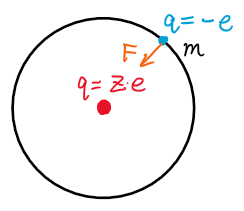
\includegraphics[width=4cm]{./figures/QMIntr1.png}
\caption{类氢原子} \label{QMIntr_fig1}
\end{figure}

\begin{equation}
\begin{aligned}
F &= \frac{1}{4\pi \epsilon_0} \frac{(Ze)e}{r^2}
\\
F &= ma = m\frac{v^2}{r}
\end{aligned}
\end{equation}

角动量量子化条件
\begin{equation}
L = mvr = n\hbar
\end{equation}
可以理解为驻波条件
\begin{equation}
2\pi r = n \lambda = n \frac{h}{mv}
\end{equation}

能级公式

\begin{equation}
E_n =  - \frac{m k e^4}{2 \hbar ^2} \frac{Z^2}{n^2} \approx - 13.6\Si{eV} \frac{Z^2}{n^2}
\qquad (n = 1, 2, \dots)
\end{equation}

\subsection{势垒散射\ 隧道效应}
参考词条\upref{QM0}

\subsection{无限深势阱}
参考词条\upref{QM0}, \href{http://wuli.wiki/apps/QMISW.html}{互动演示}
